\vspace{2mm}
\tikzset{every picture/.style={line width=0.75pt}} %set default line width to 0.75pt        

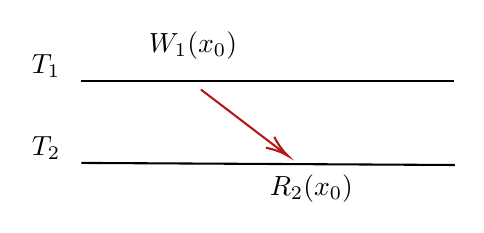
\begin{tikzpicture}[x=0.75pt,y=0.75pt,yscale=-1,xscale=1]
%uncomment if require: \path (0,300); %set diagram left start at 0, and has height of 300

%Straight Lines [id:da9351620672631715] 
\draw    (70.33,79.67) -- (250.33,79.67) ;
%Straight Lines [id:da20316716985592453] 
\draw    (70.67,119.33) -- (250.67,120.33) ;
%Straight Lines [id:da3663864520178606] 
\draw [color={rgb, 255:red, 179; green, 23; blue, 23 }  ,draw opacity=1 ]   (128.33,84) -- (168.74,114.79) ;
\draw [shift={(170.33,116)}, rotate = 217.3] [color={rgb, 255:red, 179; green, 23; blue, 23 }  ,draw opacity=1 ][line width=0.75]    (10.93,-3.29) .. controls (6.95,-1.4) and (3.31,-0.3) .. (0,0) .. controls (3.31,0.3) and (6.95,1.4) .. (10.93,3.29)   ;

% Text Node
\draw (45.33,65.67) node [anchor=north west][inner sep=0.75pt]   [align=left] {$T_1$};
% Text Node
\draw (45.33,105) node [anchor=north west][inner sep=0.75pt]   [align=left] {$T_2$};
% Text Node
\draw (101.67,54.67) node [anchor=north west][inner sep=0.75pt]   [align=left] {$W_1(x_0)$};
% Text Node
\draw (160,123.67) node [anchor=north west][inner sep=0.75pt]   [align=left] {$R_2(x_0)$};

\end{tikzpicture}
\vspace{2mm}